\documentclass[11pt]{article}
\usepackage[letterpaper,margin=0.92in]{geometry}
\usepackage{amsmath,amssymb,amsthm,mathtools}
\usepackage{booktabs,array,longtable,graphicx}
\usepackage{microtype}
\usepackage{enumitem}
\usepackage{xcolor}
\usepackage{tikz}
\usetikzlibrary{arrows.meta,positioning,calc}
\usepackage[hidelinks]{hyperref}
\usepackage{url}
\usepackage{fancyhdr}
\usepackage{lastpage}

\definecolor{darkblue}{RGB}{22,58,99}
\hypersetup{colorlinks=true,linkcolor=darkblue,citecolor=darkblue,urlcolor=darkblue}
\setlist{nosep,leftmargin=2em}
\setlength{\parskip}{0.33em}
\setlength{\parindent}{1.35em}
\setlength{\headheight}{14pt}
\setlength{\emergencystretch}{2em}
\allowdisplaybreaks

\newtheorem{theorem}{Theorem}[section]
\newtheorem{proposition}[theorem]{Proposition}
\newtheorem{lemma}[theorem]{Lemma}
\newtheorem{corollary}[theorem]{Corollary}
\newtheorem{definition}[theorem]{Definition}
\newtheorem{remark}[theorem]{Remark}
\newtheorem{audit}[theorem]{Audit proposition}

\newcommand{\Thetao}{\Theta}
\newcommand{\R}{\mathbb R}
\newcommand{\e}{\mathrm e}
\newcommand{\dd}{\,\mathrm d}
\newcommand{\Proc}{F_{\mathrm{proc}}}
\newcommand{\Table}{F_{\mathrm{table}}}
\newcommand{\Src}{F_{\mathrm{src}}}

\pagestyle{fancy}
\fancyhf{}
\lhead{Global identifiability in a three-taxon LGT model}
\rhead{Version 0.2 -- prepared for author audit}
\cfoot{\thepage\ of \pageref{LastPage}}

\title{\bfseries Global Identifiability in a Three-Taxon\\
Lateral-Gene-Transfer Model\\[0.35em]
\large An exhaustive genealogy calculation under JC69}
\author{Alec Kriebel}
\date{Version 0.2 -- prepared for author audit -- August 2026}

\begin{document}
\maketitle

\begin{abstract}
A finite enumeration of gene histories can fail for a lateral-gene-transfer process even when it reproduces the correct gene-tree topology frequencies.  After the first sampled-gene coalescence below the first species divergence, a transfer from a species branch carrying no currently traced sampled ancestry into an occupied recipient moves one sampled ancestral lineage without causing a coalescence.  Repeated movements of this kind can change the second gene-tree coalescence time and hence the JC69 branch lengths.  We sum them exhaustively by a three-state continuous-time Markov chain.

For every fixed known substitution rate $\mu>0$, the resulting parameter map for the rooted clocklike three-taxon tree $((1,2),3)$ is globally injective on $0<t_1<t_2$ and $\lambda>0$.  Its Jacobian has full rank three at every interior point, so there is neither an exceptional interior set nor a second interior preimage.  The exact distribution also identifies the rooted species-tree cherry through the strict inequality $p_{12}>p_{13}=p_{23}$.  If $\mu$ is unknown, only the usual common time-rate scale remains unidentifiable.

We also show that two finite-history formula maps associated with the model are distinct from the exhaustive stochastic-process map: one has a certified regular double point, while the other reverses the process's strict matching-pair inequality at an exact interior parameter point.  The three maps and their implications are stated separately, with deterministic symbolic and directed-rounding verification.
\end{abstract}

\tableofcontents

\section{Introduction and main results}\label{sec:introduction}

Lateral gene transfer (LGT) creates gene histories that need not follow the topology or branch lengths of a species tree.  A basic stochastic model places transfers on contemporaneous species branches according to a Poisson process, retains the donor copy, and replaces the recipient ortholog.  Kubatko, Linz, and Wicke recently derived three-taxon gene-tree and JC69 site-pattern formulas for this setting and posed a global parameter-identifiability question after proving generic local identifiability for their displayed formula map~\cite{KLW2026}.  The present paper addresses the underlying backward-lineage process directly.

The key issue is that ``relevant transfer'' cannot be equated with ``transfer that immediately coalesces two currently traced sampled lineages.''  Once the first sampled pair has coalesced, a transfer can move one of the two remaining sampled ancestral lineages through the third species branch without changing the already formed cherry.  Such a movement can decide whether the two surviving lineages meet vertically at time $t_1$ or continue toward $t_2$.  A finite list that terminates after two immediately coalescing transfers therefore need not determine the site-pattern distribution.

We distinguish three maps throughout:
\begin{enumerate}[label=\textbf{M\arabic*.}]
\item $\Proc$: the exhaustive map induced by the ordered-pair Poisson LGT process defined in Section~\ref{sec:model};
\item $\Table$: the auxiliary fourteen-history map specified in Section~\ref{sec:comparison}, with the two one-transfer density types distinguished and the displayed transfer variables treated as absolute gene-tree times;
\item $\Src$: the formula/code map distributed with arXiv:2607.14653v1 and repository commit \path{1954b2ab92525dfdaf43b50f97dcf46658cab6c9}.
\end{enumerate}
These are different analytic maps.  The principal biological theorem concerns $\Proc$ under the specific process convention below; no claim is made that this convention exhausts every possible interpretation of an LGT model.

Let
\[
\Thetao=\{(t_1,t_2,\lambda):0<t_1<t_2,\ \lambda>0\}.
\]
The site-pattern coordinates are the five aggregate equality classes
\[
(p_0,p_{12},p_{13},p_{23},p_D),
\]
where $p_0$ is the all-equal class, $p_{ij}$ is the class in which exactly taxa $i,j$ agree, and $p_D$ is the all-distinct class.

\begin{theorem}[Global process identifiability]\label{thm:primary}
Fix a known substitution rate $\mu>0$.  Consider one sampled ortholog from each taxon on the rooted clocklike species tree $((1,2),3)$, with $0<t_1<t_2$, no incomplete lineage sorting, constant ordered-pair transfer-rate parameter $\lambda>0$, donor retention, recipient replacement, and the backward-lineage process of Section~\ref{sec:model}.  Under JC69, the exact population site-pattern distribution uniquely determines $(t_1,t_2,\lambda)$.

Equivalently, $\Proc$ is globally injective on $\Thetao$.  Its distributional Jacobian has rank three at every interior point.  Thus there is no exceptional interior set and no second interior parameter preimage.
\end{theorem}

The theorem is stronger than generic identifiability.  It is proved by reducing each fixed pair of observed coordinates to a single formal one-dimensional inverse branch, proving that its physically feasible part is an interval, and showing that the third observed coordinate is strictly monotone along that interval.

\begin{corollary}[Joint topology-and-parameter identifiability]\label{cor:topology}
Among the three labeled rooted clocklike three-taxon species trees, the exact JC69 site-pattern distribution under the ordered-pair Poisson LGT process jointly identifies the rooted species-tree topology and, conditional on that topology, uniquely identifies $(t_1,t_2,\lambda)$ for every fixed known $\mu>0$.
\end{corollary}

The result has a necessary rate-scale qualification.

\begin{proposition}[Unknown-rate scale ambiguity]\label{prop:scale}
If $\mu$ is also treated as unknown, then for every $c>0$ the transformation
\[
(t_1,t_2,\lambda,\mu)
\longmapsto
(ct_1,ct_2,\lambda/c,\mu/c)
\]
leaves the entire site-pattern distribution unchanged.  Consequently, $t_1,t_2,\lambda,$ and $\mu$ cannot be jointly identified without fixing a time or rate scale.
\end{proposition}

Two secondary results clarify why formulas associated with a finite history reduction do not settle the process theorem.

\begin{proposition}[Regular double point of the auxiliary map]\label{prop:table}
The auxiliary map $\Table$ is not generically identifiable in the measure-zero-exception sense.  More precisely, its image contains a nonempty open set of regular observed distributions such that every distribution in that set has at least two distinct preimages under $\Table$.
\end{proposition}

\begin{audit}[Exact diagnostic for the distributed source map]\label{prop:source}
For arXiv:2607.14653v1 and repository commit \texttt{1954b2ab92525dfdaf43b50f97dcf46658cab6c9}, the distributed formula/code map $\Src$ is distinct from both $\Proc$ and $\Table$.  At the exact admissible cube point
\[
(q,x,y)=\left(\frac12,\frac{81}{100},\frac1{10}\right),
\]
it produces a strictly positive normalized aggregate distribution but satisfies
\[
A_{\rm src}-B_{\rm src}=-\frac{57472173}{800000000}<0,
\qquad
p_{12}^{\rm src}-p_{13}^{\rm src}
=-\frac{172416519}{3200000000}<0.
\]
Thus it reverses the strict matching-pair inequality satisfied by $\Proc$.
\end{audit}

The source paper's conjecture is formally attached to its displayed parameter map.  Theorem~\ref{thm:primary} therefore should not be paraphrased as an unqualified proof of that formula-level conjecture.  Rather, it gives a stronger positive answer to the intended stochastic-process identifiability question after the induced genealogy measure is summed exhaustively.  The distributed formula must be reconciled with the process before formula-based identifiability or inference claims can be interpreted as statements about that process.

\paragraph{Scope.}
Theorem~\ref{thm:primary} assumes: one sampled ortholog per taxon; a rooted clocklike three-taxon species tree; one constant ordered-pair rate $\lambda$; the donor-retains, recipient-replaced backward-lineage convention below; JC69 substitution; fixed known $\mu>0$; no incomplete lineage sorting; and exact population site-pattern probabilities.  It does not cover unknown $\mu$ without a fixed scale, joint LGT--ILS models, larger taxon sets, finite-sample guarantees, branch-specific or distance-dependent transfer rates, or alternative transfer conventions.

\section{Model definition and notation}\label{sec:model}

\subsection{Species tree and ordered-pair transfer process}
The species tree is $((1,2),3)$, with leaves at time zero, the $1$--$2$ divergence at time $t_1$, and the root divergence at time $t_2$.  There are three contemporaneous species branches during $(0,t_1)$ and two during $(t_1,t_2)$.

When $k$ species branches are present, transfers occur at total rate $k\lambda$.  Conditional on a transfer, an ordered donor--recipient pair is chosen uniformly among the $k(k-1)$ possibilities.  Hence every ordered pair has rate $\lambda/2$ below $t_1$ and rate $\lambda$ above $t_1$.  Forward in time, the donor retains its copy and the transferred copy replaces the recipient ortholog.

Tracing the three sampled genes backward, a lineage on a recipient branch follows the transfer arc to the donor branch.  A transfer can be irrelevant, can move a sampled ancestral lineage without coalescence, or can coalesce two sampled ancestral lineages.  Events are almost surely at distinct times.

\begin{definition}[Ancestrally unoccupied species branch]\label{def:unoccupied}
A species branch is called \emph{ancestrally unoccupied} when it currently carries none of the ancestral lineages of the sampled leaf genes.  The branch still carries a population gene copy.  ``Unoccupied'' refers only to the induced genealogy of the sampled genes.
\end{definition}

After Definition~\ref{def:unoccupied}, the phrase \emph{empty state} is used only as shorthand for the identity of the ancestrally unoccupied species branch.

\subsection{JC69 mutation process}
The root state is uniform on four nucleotides.  Along an edge of length $s$,
\[
P_{ii}(s)=\frac14+\frac34\e^{-\mu s},
\qquad
P_{ij}(s)=\frac14-\frac14\e^{-\mu s}\quad(i\ne j),
\]
with fixed known $\mu>0$.  Conditional on the gene tree, mutations on distinct edges are independent.  The normalization $\mu=4/3$ is used in the exact numerical certificates, while all process-identifiability arguments below are valid for arbitrary fixed $\mu>0$.

\section{The missing noncoalescing movement mechanism}\label{sec:missing}

The omission can be seen in a two-transfer path.  Let time increase backward from the leaves and choose
\[
0<u<v<t_1.
\]
At time $u$, branch $1$ transfers into branch $2$.  Backward in time, the sampled lineage from taxon $2$ jumps to branch $1$ and coalesces with the sampled lineage from taxon $1$.  The sampled pair $(1,2)$ has now formed the cherry.  The two surviving sampled ancestral lineages occupy branches $1$ and $3$, while branch $2$ is ancestrally unoccupied.

At time $v$, branch $2$ transfers into branch $3$.  Backward in time, the lineage on recipient branch $3$ jumps to donor branch $2$.  This transfer causes no immediate sampled-gene coalescence.  The surviving sampled lineages now occupy branches $1$ and $2$, and therefore coalesce vertically at $t_1$.  Without the second transfer, they would have remained on branches $1$ and $3$ and would not coalesce at $t_1$.

\begin{figure}[ht]
\centering
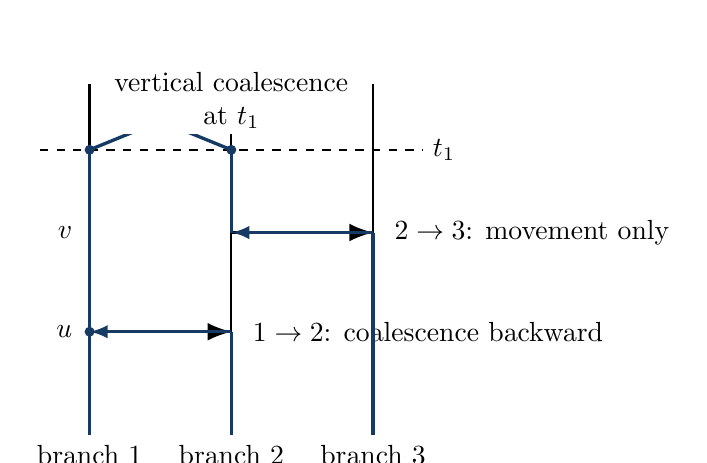
\begin{tikzpicture}[x=1.8cm,y=1.05cm,>=Latex,thick]
  \draw (0,0) -- (0,4.25);
  \draw (1,0) -- (1,4.25);
  \draw (2,0) -- (2,4.25);
  \node[below] at (0,0) {branch 1};
  \node[below] at (1,0) {branch 2};
  \node[below] at (2,0) {branch 3};
  \draw[dashed] (-0.35,3.45) -- (2.35,3.45);
  \node[right] at (2.35,3.45) {$t_1$};
  \draw[-{Latex[length=3mm]}] (0,1.25) -- (1,1.25);
  \node[left] at (-0.05,1.25) {$u$};
  \node[anchor=west] at (1.08,1.25) {$1\to2$: coalescence backward};
  \draw[-{Latex[length=3mm]}] (1,2.45) -- (2,2.45);
  \node[left] at (-0.05,2.45) {$v$};
  \node[anchor=west] at (2.08,2.45) {$2\to3$: movement only};
  \draw[very thick,darkblue] (0,0) -- (0,3.45);
  \draw[very thick,darkblue] (1,0) -- (1,1.25);
  \draw[very thick,darkblue] (2,0) -- (2,2.45);
  \draw[very thick,darkblue,-{Latex[length=2.3mm]}] (2,2.45) -- (1,2.45);
  \draw[very thick,darkblue] (1,2.45) -- (1,3.45);
  \fill[darkblue] (0,1.25) circle (1.8pt);
  \draw[very thick,darkblue,-{Latex[length=2.3mm]}] (1,1.25) -- (0,1.25);
  \fill[darkblue] (0,3.45) circle (1.8pt);
  \fill[darkblue] (1,3.45) circle (1.8pt);
  \draw[very thick,darkblue] (0,3.45) -- (0.5,3.8) -- (1,3.45);
  \node[align=center,fill=white,inner sep=2pt] at (1.0,4.05) {vertical coalescence\\at $t_1$};
\end{tikzpicture}
\caption{A transfer that is noncoalescing at time $v$ changes whether the two surviving sampled lineages coalesce vertically at $t_1$.  The already formed cherry remains $(1,2)$.  Arrows show forward donor-to-recipient directions; the sampled lineage follows them backward.}
\label{fig:movement}
\end{figure}

This example establishes four distinct points: the second transfer changes the sampled genealogy; it does not itself cause a coalescence; it changes the second coalescence time and branch lengths; and it does not change the sampled pair that already formed the cherry.  Consequently, topology-frequency formulas can remain correct while site-pattern probabilities are wrong.  Under the backward-lineage interpretation defined in Section~\ref{sec:model}, a fourteen-history list that omits such repeated movements is not exhaustive.

\section{Exhaustive genealogy measure}\label{sec:genealogy}

\subsection{The post-coalescence three-state chain}
Before the first sampled-gene coalescence below $t_1$, all three species branches are ancestrally occupied.  Every transfer then coalesces one sampled pair, so the first coalescence time has rate $3\lambda$ and each unordered sampled pair is selected with probability $1/3$.

Suppose the first coalescence occurs at absolute time $u<t_1$.  Two sampled ancestral lineages remain.  Let $E\in\{1,2,3\}$ denote the empty state.  For a fixed $E=e$:
\begin{itemize}
\item the two ordered transfers between occupied branches have combined rate $\lambda$ and absorb the process by coalescing the surviving lineages;
\item the two transfers whose donor is branch $e$ and whose recipient is occupied have combined rate $\lambda$ and move the empty state, each at rate $\lambda/2$;
\item transfers whose recipient is branch $e$ have combined rate $\lambda$ and leave the induced sampled genealogy unchanged.
\end{itemize}
The absorption hazard is $\lambda$, independent of the empty state.  Conditional on nonabsorption, $E$ has generator
\begin{equation}\label{eq:Q}
Q=\frac{\lambda}{2}
\begin{pmatrix}
-2&1&1\\
1&-2&1\\
1&1&-2
\end{pmatrix}.
\end{equation}

\begin{lemma}[Post-coalescence transition kernel]\label{lem:ctmc}
For elapsed time $s\ge0$, the probability of no second transfer-coalescence is $\e^{-\lambda s}$.  Conditional on this survival,
\[
P_{ee}(s)=\frac13+\frac23\e^{-3\lambda s/2},
\qquad
P_{ee'}(s)=\frac13-\frac13\e^{-3\lambda s/2}\quad(e'\ne e).
\]
\end{lemma}
\begin{proof}
The absorption clock of rate $\lambda$ is independent of the movement chain.  The matrix $Q$ has eigenvalue $0$ on the constant vector and eigenvalue $-3\lambda/2$ on its orthogonal complement.  Exponentiating $Q$ gives the displayed kernel.
\end{proof}

\subsection{Disjoint history classes}
Write
\[
T_1=((1,2),3),\qquad T_2=((1,3),2),\qquad T_3=((2,3),1).
\]
The first transfer below $t_1$, when present, fixes the sampled cherry and hence the gene-tree topology.

If no transfer occurs before $t_1$, its probability is $\e^{-3\lambda t_1}$ and taxa $1,2$ coalesce vertically at $t_1$.  Above $t_1$, the remaining two lineages coalesce at a transfer time $v\in(t_1,t_2)$ with density
\[
2\lambda\e^{-\lambda(t_1+2v)},
\]
or at $t_2$ with point mass $\e^{-\lambda(t_1+2t_2)}$.

If the first coalescence occurs at $u\in(0,t_1)$, then for each topology $T_i$ its aggregate first-event density is
\[
\lambda\e^{-3\lambda u}.
\]
A second transfer-coalescence at $v\in(u,t_1)$ has, for each $T_i$, joint density
\begin{equation}\label{eq:below-density}
\lambda^2\e^{-\lambda(2u+v)},\qquad 0<u<v<t_1.
\end{equation}
Indeed, after the first event, survival from $u$ to $v$ is $\e^{-\lambda(v-u)}$, followed by absorption density $\lambda$.

For histories surviving to $t_1$, define
\[
b(u)=\lambda\e^{-\lambda(t_1+2u)},
\qquad
\rho_u=\e^{-3\lambda(t_1-u)/2}.
\]
The topology-dependent probabilities of vertical coalescence at $t_1$ and continuation above $t_1$ are
\begin{center}
\begin{tabular}{c|cc}
\toprule
Topology & coalesce at $t_1$ & continue above $t_1$\\
\midrule
$T_1$ & $(1-\rho_u)/3$ & $(2+\rho_u)/3$\\
$T_2$ & $(2+\rho_u)/6$ & $(4-\rho_u)/6$\\
$T_3$ & $(2+\rho_u)/6$ & $(4-\rho_u)/6$\\
\bottomrule
\end{tabular}
\end{center}
Multiplication by $b(u)$ gives the corresponding measure at $t_1$.  Conditional on continuation, the second coalescence occurs at $v\in(t_1,t_2)$ with density $2\lambda\e^{-2\lambda(v-t_1)}$, or at $t_2$ with mass $\e^{-2\lambda(t_2-t_1)}$.

\begin{proposition}[Exhaustiveness, normalization, and topology probabilities]\label{prop:history}
The cases above are mutually exclusive and exhaustive for the sampled-gene genealogy under the process of Section~\ref{sec:model}.  Their total mass is one.  Summing by topology gives
\[
\Pr(T_1)=\frac13+\frac23\e^{-3\lambda t_1},
\qquad
\Pr(T_2)=\Pr(T_3)=\frac13-\frac13\e^{-3\lambda t_1}.
\]
All integration variables in this genealogy measure are absolute times.
\end{proposition}
\begin{proof}
Either there is no transfer before $t_1$, or the first transfer occurs at a unique $u<t_1$.  In the latter event, the residual process either absorbs at a unique $v<t_1$ or survives to $t_1$.  On survival, the two lineages either coalesce vertically at $t_1$ or continue; a continuing pair either transfers before $t_2$ or coalesces vertically at $t_2$.  The memoryless construction makes these alternatives disjoint and exhaustive.

At the first level,
\[
\e^{-3\lambda t_1}
+\sum_{i=1}^{3}\int_0^{t_1}\lambda\e^{-3\lambda u}\dd u=1.
\]
Lemma~\ref{lem:ctmc}, the row sums of the displayed table, and the two-lineage exponential law above $t_1$ each have conditional mass one.  The topology formulas follow because no transfer below $t_1$ forces $T_1$, whereas a first transfer below $t_1$ chooses each unordered pair with probability $1/3$.
\end{proof}

\section{Fourier coordinates and the corrected parameter map}\label{sec:map}

\subsection{Conditional JC69 coordinates}
Identify the four states with $G=\mathbb Z_2^2$.  For a nontrivial character $\chi$ of $G$,
\[
\mathbb E[\chi(X_s)\mid X_0]=\e^{-\mu s}\chi(X_0).
\]
A uniform root kills Fourier moments whose character product is nontrivial.

\begin{proposition}[Three-leaf ultrametric gene tree]\label{prop:fourier-tree}
Let a three-leaf ultrametric gene tree have interior times $0<g_1<g_2$.  If $i,j$ form its cherry, then
\[
\widehat p_{ij}=\e^{-2\mu g_1},
\qquad
\widehat p_{ik}=\widehat p_{jk}=\e^{-2\mu g_2}.
\]
For three nontrivial characters whose product is trivial,
\[
\widehat p_{123}=\e^{-\mu(g_1+2g_2)}.
\]
\end{proposition}
\begin{proof}
A pair moment propagates along the path joining the two leaves, of length $2g_1$ for the cherry and $2g_2$ otherwise.  In the three-way moment, the three pendant edges and the internal cherry edge carry nontrivial characters.  Their total contributing length is
$g_1+g_1+g_2+(g_2-g_1)=g_1+2g_2$.
\end{proof}

\subsection{Aggregate patterns and Fourier observables}
Let $p_0$ be the aggregate probability of three equal states; let $p_{12}$, $p_{13}$, and $p_{23}$ be the aggregate probabilities that exactly the named pair agrees; and let $p_D$ be the all-distinct aggregate.  For topology $((1,2),3)$, symmetry gives $p_{13}=p_{23}$ and
\[
p_0+p_{12}+2p_{13}+p_D=1.
\]
Define
\[
A=\frac{4(p_0+p_{12})-1}{3},\qquad
B=\frac{4(p_0+p_{13})-1}{3},\qquad
C=\frac{16p_0-1-3A-6B}{6}.
\]

\begin{proposition}[Exact coordinate equivalence]\label{prop:site-fourier}
The inverse transformation is
\begin{align*}
p_0&=\frac{1+3A+6B+6C}{16},\\
p_{12}&=\frac{3(1+3A-2B-2C)}{16},\\
p_{13}=p_{23}&=\frac{3(1-A+2B-2C)}{16},\\
p_D&=\frac{3(1-A-2B+2C)}8.
\end{align*}
Thus exact site-pattern identifiability is equivalent to identifiability from $(A,B,C)$.  Moreover,
\begin{equation}\label{eq:pattern-diff}
A-B=\frac43(p_{12}-p_{13}).
\end{equation}
\end{proposition}
\begin{proof}
Direct substitution in both directions gives the identity on the affine hyperplane $p_0+p_{12}+2p_{13}+p_D=1$.  Subtracting the definitions of $A$ and $B$ gives \eqref{eq:pattern-diff}.
\end{proof}

\subsection{Cube reparameterization}
For fixed $\mu>0$, set
\begin{equation}\label{eq:cube}
q=\frac{\lambda}{\lambda+\mu},\qquad
x=\e^{-(\lambda+\mu)t_1},\qquad
y=\e^{-(\lambda+\mu)(t_2-t_1)}.
\end{equation}
This is a bijection from $\Thetao$ to $(0,1)^3$, with inverse
\begin{equation}\label{eq:cube-inverse}
\lambda=\frac{\mu q}{1-q},\qquad
t_1=-\frac{1-q}{\mu}\log x,\qquad
t_2=t_1-\frac{1-q}{\mu}\log y.
\end{equation}
Define
\[
r=q+(1-q)y^2,\qquad X=x^{2-q},\qquad Z=x^3,
\]
and observable combinations
\[
D=A-B,\qquad M=\frac{A+2B}{3}.
\]
The linear change $(A,B,C)\leftrightarrow(D,M,C)$ is invertible, with
$A=M+2D/3$ and $B=M-D/3$.

\begin{theorem}[Compact exhaustive-process map]\label{thm:compact}
Averaging Proposition~\ref{prop:fourier-tree} over the exhaustive genealogy measure gives
\begin{align}
D&=(1-r)x^{2+q/2},\label{eq:D}\\
M&=\frac{q(1-X)}{2-q}+\frac{1+2r}{3}X,\label{eq:M}\\
C&=\frac{q^2\{(q-2)Z+3X-(q+1)\}}{(q-2)(q+1)}
+rZ+\frac{q(1+2r)}{q+1}(X-Z).\label{eq:C}
\end{align}
The transformed domain is
\[
0<q<1,\qquad 0<x<1,\qquad q<r<1.
\]
In particular,
\begin{equation}\label{eq:Dpositive}
A-B=(1-q)(1-y^2)x^{2+q/2}>0.
\end{equation}
The formulas are independent of the numerical value of fixed $\mu$ after the reparameterization \eqref{eq:cube}.
\end{theorem}
\begin{proof}
Appendix~\ref{app:integration} integrates every disjoint genealogy class in absolute time.  Substituting $\lambda=q(\lambda+\mu)$, $\mu=(1-q)(\lambda+\mu)$, and \eqref{eq:cube} into the resulting original-parameter map reduces all exponentials to powers of $x,y$.  Collecting $D$, $M$, and $C$ gives \eqref{eq:D}--\eqref{eq:C}.  The deterministic verifier performs the same history-by-history integration symbolically and independently checks the simplification.
\end{proof}

\begin{proof}[Proof of Proposition~\ref{prop:scale}]
Under the displayed scaling,
\[
\frac{\lambda/c}{\lambda/c+\mu/c}=\frac{\lambda}{\lambda+\mu}=q,
\]
while
\[
\exp\!\left[-\left(\frac{\lambda+\mu}{c}\right)ct_1\right]=x,
\qquad
\exp\!\left[-\left(\frac{\lambda+\mu}{c}\right)c(t_2-t_1)\right]=y.
\]
The compact map depends only on $(q,x,y)$, so the full distribution is unchanged.
\end{proof}

\section{Global injectivity}\label{sec:global}

The proof fixes $(D,M)$, constructs the unique formal inverse branch indexed by $q$, proves that the physically feasible $q$-values form one interval, and then shows that $C$ is strictly decreasing along that interval.

\subsection{A unique formal branch at each \texorpdfstring{$q$}{q}}
Let
\[
\alpha(q)=\frac{4+q}{2(2-q)},
\qquad
\gamma(q)=\frac{3q}{2(2-q)}.
\]
Since $D=(1-r)X^\alpha$, eliminating $r$ from \eqref{eq:M} gives
\begin{equation}\label{eq:Phi}
M=\Phi_q(X):=
\frac{q}{2-q}+\frac{2(1-q)}{2-q}X
-\frac{2D}{3}X^{-\gamma}.
\end{equation}

\begin{lemma}[Unique formal fixed-$(D,M)$ branch]\label{lem:formal}
Fix $(D,M)$ arising from an interior parameter point.  For every $q\in(0,1)$, equation \eqref{eq:Phi} has exactly one solution $X(q)\in(0,1)$.  It uniquely determines
\[
x(q)=X(q)^{1/(2-q)},
\qquad
r(q)=1-DX(q)^{-\alpha(q)}.
\]
The functions $X,x,r$ are smooth.
\end{lemma}
\begin{proof}
For $D>0$,
\[
\Phi_q'(X)=\frac{2(1-q)}{2-q}
+\frac{2D\gamma}{3}X^{-\gamma-1}>0.
\]
Furthermore, $\Phi_q(X)\to-\infty$ as $X\downarrow0$, whereas
$\Phi_q(1)=1-2D/3$.  At the generating point, $X<1$ and strict monotonicity gives $M<1-2D/3$.  Therefore a unique solution lies in $(0,1)$ for every $q$.  The implicit function theorem gives smoothness.
\end{proof}

\subsection{The physically feasible \texorpdfstring{$q$}{q}-set is an interval}
Along the formal branch, put
\[
p=2-q\in(1,2),\qquad \tau=-\log x>0,
\qquad h(q)=\frac{1-r(q)}{1-q}.
\]
At a physical point, $h=1-y^2$.

\begin{lemma}[Feasible-interval lemma]\label{lem:feasible}
The set of $q\in(0,1)$ for which the fixed-$(D,M)$ formal branch is physical is a nonempty interval.
\end{lemma}
\begin{proof}
We make each sign and crossing step explicit.

First, equation \eqref{eq:D} and $D>0$ imply $1-r(q)>0$ on the entire formal branch, hence $r(q)<1$.  Since $1-q>0$, it follows that $h(q)>0$ for every formal $q$.  Physical feasibility is
\[
q<r(q)<1
\quad\Longleftrightarrow\quad
0<h(q)<1.
\]
Indeed, $r=1-(1-q)h$.

Implicit differentiation of the fixed-$D,M$ equations in variables $(p,\tau,h)$ gives
\begin{equation}\label{eq:hp}
\frac{\dd h}{\dd p}
=-\frac{hN}{p^2(p-1)\{h(p-2)-2\}},
\end{equation}
where
\begin{align*}
N={}&hp^2\{2(p-1)\tau+p-2\}-6p(p-1)\tau\\
&\quad +(p-6)\e^{p\tau}-2p^2-p+6.
\end{align*}
For $1<p<2$, $\tau>0$, and $0<h\le1$, set
$B_0=2(p-1)\tau+p-2$.  If $B_0<0$, then $hp^2B_0<0$ and, because $p-6<0$ and $\e^{p\tau}>1$,
\[
N<-6p(p-1)\tau-2p^2<0.
\]
If $B_0\ge0$, use $h\le1$ and the same exponential bound to obtain
\[
N<2p(p-1)(p-3)\tau+p^2(p-4)<0.
\]
The denominator in \eqref{eq:hp} is negative, so $\dd h/\dd p<0$, equivalently
\begin{equation}\label{eq:hqpositive}
\frac{\dd h}{\dd q}>0\qquad\text{whenever }h\le1.
\end{equation}

Thus every crossing of the level $h=1$ is from below to above.  If a branch that had left $h<1$ later re-entered it, continuity would force a downward crossing of $h=1$, contradicting \eqref{eq:hqpositive}.  Hence $\{q:h(q)<1\}$ is an interval.  Since $h(q)>0$ everywhere, this is exactly the feasible set $\{q:0<h(q)<1\}$.  The observed generating point belongs to it, so the interval is nonempty.
\end{proof}

\subsection{Strict Jacobian orientation}
The relevant $(x,r)$ minor is
\begin{equation}\label{eq:minor}
\det\frac{\partial(D,M)}{\partial(x,r)}
=x^{3-q/2}\{2-q(1+r)\}>0,
\end{equation}
because $0<q,r<1$.

To determine the full determinant, retain $p=2-q$, set $X=\e^{-s}$, and write $r=1-(p-1)h$, with
\[
1<p<2,\qquad s>0,\qquad 0<h<1.
\]
The exact factorization is
\begin{equation}\label{eq:detfactor}
\det\frac{\partial(D,M,C)}{\partial(p,X,r)}
=\frac{(p-1)^2X^{3/p-3/2}}{p^3(3-p)^2}
\e^{-(1+3/p)s}\mathcal H(s),
\end{equation}
where
\begin{align*}
\mathcal H(s)&=\beta\e^{3s/p}+\gamma_0\e^s
+\alpha\e^{(3/p-1)s}+\delta+\eta s,\\
\alpha&=-2p(hp-3)(hp-2h-2)<0,\\
\beta&=-p(p-3)(p-2)(hp-2h-2)>0,\\
\gamma_0&=(p-3)(hp-6)>0,\\
\eta&=(3-p)(p-1)(ph^2-3ph+6)>0,\\
\delta&=-\alpha-\beta-\gamma_0.
\end{align*}

\begin{lemma}[Positivity of the determinant factor]\label{lem:Hpositive}
For $1<p<2$, $0<h<1$, and $s>0$, one has $\mathcal H(s)>0$.
\end{lemma}
\begin{proof}
The initial values are
\[
\mathcal H(0)=0,
\qquad
\mathcal H'(0)=ph^2(3-p)^2>0.
\]
Put $a_0=(3-p)/p$ and
\[
\mathcal J(s)=\e^{-a_0s}\mathcal H''(s)
=\frac{9\beta}{p^2}\e^s
+\gamma_0\e^{(2-3/p)s}+\alpha a_0^2.
\]
At zero,
\[
\mathcal J(0)=-2h(p-3)^2(hp-2h-1)>0.
\]
If $p\ge3/2$, then $2-3/p\ge0$ and $\mathcal J'(s)>0$.  If $p<3/2$, then
\[
\mathcal J''(s)=\frac{9\beta}{p^2}\e^s
+(2-3/p)^2\gamma_0\e^{(2-3/p)s}>0
\]
and
\[
\mathcal J'(0)=-\frac{(p-3)^2}{p}(7hp-12h-6)>0,
\]
since $7p-12<0$.  Hence $\mathcal J(s)>0$ in both cases.  Therefore $\mathcal H''(s)>0$, and the initial values imply $\mathcal H(s)>0$ for all $s>0$.
\end{proof}

All remaining factors in \eqref{eq:detfactor} are positive.  The coordinate change $(q,x,r)\mapsto(p,X,r)$ has determinant
\[
-px^{p-1}<0.
\]
Consequently,
\begin{equation}\label{eq:jacnegative}
\det\frac{\partial(D,M,C)}{\partial(q,x,r)}<0
\end{equation}
throughout the domain.  Since $\partial r/\partial y=2(1-q)y>0$, the determinant in $(q,x,y)$ coordinates is also strictly negative.

\subsection{Strict monotonicity of the final coordinate}
Along the fixed-$(D,M)$ branch, Cramer's rule and \eqref{eq:minor} give
\begin{equation}\label{eq:Cmonotone}
\frac{\dd C}{\dd q}
=\frac{\det\{\partial(D,M,C)/\partial(q,x,r)\}}
       {\det\{\partial(D,M)/\partial(x,r)\}}<0.
\end{equation}
By Lemma~\ref{lem:feasible}, the physical branch is an interval; hence $C$ is strictly decreasing on its whole feasible part.

\begin{proof}[Proof of Theorem~\ref{thm:primary}]
Suppose two interior parameter points have the same site-pattern distribution.  Proposition~\ref{prop:site-fourier} gives the same $(D,M,C)$.  Lemma~\ref{lem:formal} places both on the unique formal fixed-$(D,M)$ branch, and Lemma~\ref{lem:feasible} places both $q$-values in one feasible interval.  Strict monotonicity \eqref{eq:Cmonotone} forces the same $q$.  Lemma~\ref{lem:formal} then forces the same $X,r$, hence the same $x,y$.  The inverse \eqref{eq:cube-inverse} gives the same $(t_1,t_2,\lambda)$.

Equation \eqref{eq:jacnegative}, the positive derivative $\partial r/\partial y$, the invertible observable-coordinate change, the affine site-pattern transformation, and the cube diffeomorphism prove full rank of the distributional Jacobian everywhere in $\Thetao$.
\end{proof}

\paragraph{Constructive inversion.}
Given an exact interior distribution, compute $D,M,C$.  For each trial $q$, solve the strictly increasing scalar equation $\Phi_q(X)=M$; set $r=1-DX^{-\alpha(q)}$; retain the unique interval on which $q<r<1$; and solve the strictly decreasing equation $C(q)=C_{\rm obs}$.  Finally set
\[
x=X^{1/(2-q)},\qquad y=\sqrt{\frac{r-q}{1-q}},
\]
and apply \eqref{eq:cube-inverse}.  The final scalar root generally is transcendental, but it is globally unambiguous.

\section{Joint topology-and-parameter identifiability}\label{sec:topology}

\begin{proof}[Proof of Corollary~\ref{cor:topology}]
For species topology $((1,2),3)$, Theorem~\ref{thm:compact} gives
\[
D=A-B=(1-r)x^{2+q/2}>0.
\]
By \eqref{eq:pattern-diff},
\[
p_{12}>p_{13}=p_{23}.
\]
After relabeling, the exactly equal discordant-pair probabilities and the uniquely largest matching-pair probability identify the species-tree cherry.  Once the labels are arranged so the topology is $((1,2),3)$, Theorem~\ref{thm:primary} uniquely identifies $(t_1,t_2,\lambda)$.
\end{proof}

The strict inequality holds at every interior point; equality occurs only on boundary degenerations such as $t_2\downarrow t_1$.  This topology result is therefore global on the open model domain, not merely generic.

\section{Statistical interpretation and conditioning}\label{sec:statistics}

Global population identifiability does not imply uniform finite-sample stability.  For example, as $t_2-t_1\downarrow0$, equation \eqref{eq:Dpositive} gives $D\downarrow0$, so the topology signal and a direction of the inverse become ill-conditioned.  Extreme transfer-rate or divergence-time regimes can likewise produce broad, correlated likelihood contours.  Conditioning and finite-sample error require separate analysis.

The regular-double-point statement for $\Table$ has a precise population-likelihood implication, which follows from more than the inverse function theorem alone.

\begin{lemma}[Population multinomial Hessian at an exact fit]\label{lem:hessian}
Let $p(\theta)=(p_i(\theta))_{i=1}^m$ be a positive probability vector with $\sum_i p_i(\theta)=1$, and let $p^*=p(\theta_0)$.  Define the population multinomial log-likelihood
\[
\ell(\theta)=\sum_{i=1}^{m}p_i^*\log p_i(\theta).
\]
Then
\[
\nabla\ell(\theta_0)=0,
\qquad
\nabla^2\ell(\theta_0)
=-J(\theta_0)^T\operatorname{diag}(1/p_i^*)J(\theta_0),
\]
where $J$ is the distributional Jacobian.  If $J(\theta_0)$ has full column rank, the Hessian is negative definite.
\end{lemma}
\begin{proof}
At the exact fit,
\[
\nabla\ell(\theta_0)=\sum_i \nabla p_i(\theta_0)
=\nabla\sum_i p_i(\theta_0)=0.
\]
Differentiating again gives
\[
\nabla^2\ell(\theta_0)
=\sum_i\nabla^2p_i(\theta_0)
-\sum_i\frac{\nabla p_i(\theta_0)\nabla p_i(\theta_0)^T}{p_i^*}.
\]
The first sum vanishes because $\sum_i p_i(\theta)=1$.  The remaining quadratic form is strictly negative on every nonzero parameter direction when $J$ has full column rank.
\end{proof}

The two certified $\Table$ preimages have strictly positive pattern probabilities and full-rank Jacobians.  By continuity and the local inverse branches, every distribution in a sufficiently small open overlap has two separated exact-fitting parameter values, each a strict local maximizer of its corresponding population multinomial log-likelihood.  This does not imply a particular finite-sample optimizer will find both modes, nor does it establish a global fiber count outside that local overlap.

\section{Comparison with the auxiliary and distributed maps}\label{sec:comparison}

\subsection{The auxiliary fourteen-history map \texorpdfstring{$\Table$}{Ftable}}
The auxiliary map is defined by the fourteen named classes
\[
\begin{aligned}
\mathcal G_{14}=\{&G_{1x},G_{1a},G_{1b},G_{1c},G_{1d},G_{1y},\\
                    &G_{2a},G_{2b},G_{2c},G_{2d},
                      G_{3a},G_{3b},G_{3c},G_{3d}\}.
\end{aligned}
\]
It distinguishes the two discordant one-transfer density types and interprets the displayed transfer variables as absolute gene-tree times.  It is internally normalized, but under the backward-lineage interpretation of Section~\ref{sec:model} it omits the repeated noncoalescing movements of Section~\ref{sec:missing}.

With
\[
K(q)=\frac{q(2q+1)}{q+2},
\]
its cube formulas are
\begin{align}
A_{\rm table}&=K(q)+(1-q)x^2\{1+(1-x^q)y^2\}
+\frac{q(1-q)}{q+2}x^{q+2},\label{eq:Atable}\\
B_{\rm table}&=K(q)+\frac{1-q}{2}x^2\{1+(3-x^q)y^2\}
-\frac{(1-q)(2-q)}{2(q+2)}x^{q+2},\label{eq:Btable}\\
C_{\rm table}&=q^2+q(1-q)x^2+2q(1-q)x^2y^2
+(1-q)(1-2q)x^3y^2.\label{eq:Ctable}
\end{align}
It satisfies
\[
A_{\rm table}-B_{\rm table}
=\frac{1-q}{2}x^2(1+x^q)(1-y^2)>0.
\]

At
\[
z_1=(q_1,x_1,y_1)=\left(\frac12,\frac1{10},\frac35\right),
\]
the exact target is
\begin{align*}
A_0&=\frac{1017}{2500}-\frac{\sqrt{10}}{12500},\\
B_0&=\frac{1013}{2500}-\frac{3\sqrt{10}}{12500},\\
C_0&=\frac{2543}{10000}.
\end{align*}
The aggregate pattern probabilities are
\begin{align*}
p_0&=\frac{30887}{80000}-\frac{21\sqrt{10}}{200000},\\
p_{12}&=\frac{13521}{80000}+\frac{9\sqrt{10}}{200000},\\
p_{13}=p_{23}&=\frac{537}{3200}-\frac{3\sqrt{10}}{40000},\\
p_D&=\frac{4371}{40000}+\frac{21\sqrt{10}}{100000},
\end{align*}
all strictly positive.

Appendix~\ref{app:certificate} gives a rational interval box $B_2$ in which a 384-bit outward-rounded Krawczyk calculation proves the existence and uniqueness of a second root $z_2$ of
$\Table(z)=(A_0,B_0,C_0)$.  The determinant enclosures are
\begin{align*}
\det D\Table(B_2)&\subset
[-7.16842960336480910\times10^{-3},
 -7.16842960336480824\times10^{-3}],\\
\det D\Table(z_1)&\subset
[6.82019607798308635\times10^{-5},
 6.82019607798308770\times10^{-5}].
\end{align*}
Thus both preimages are regular and distinct.

\begin{lemma}[Regular double point gives an open two-sheeted overlap]\label{lem:ift}
Let $F:U\to\mathbb R^3$ be continuously differentiable on an open set.  If $z_1\ne z_2$, $F(z_1)=F(z_2)=w$, and both Jacobians are nonsingular, then there exist disjoint open neighborhoods $U_1,U_2$ and a nonempty open set $V\ni w$ such that every value in $V$ has one preimage in each $U_i$.
\end{lemma}
\begin{proof}
Choose disjoint neighborhoods of $z_1,z_2$.  The inverse function theorem permits shrinking them so that $F$ restricts to a diffeomorphism from $U_i$ onto an open neighborhood $V_i$ of $w$.  Then $V=V_1\cap V_2$ has the stated property.
\end{proof}

\begin{proof}[Proof of Proposition~\ref{prop:table}]
The directed-rounding certificate supplies the distinct regular preimages.  Lemma~\ref{lem:ift} gives a nonempty open set of regular values with at least two preimages.  Therefore no measure-zero exceptional set can restore injectivity of $\Table$ on the complement: the failure occurs over an open set.  No claim is made that almost every point in the entire image has multiple preimages or that every regular fiber has exactly two points.
\end{proof}

\subsection{The distributed formula/code map \texorpdfstring{$\Src$}{Fsrc}}
The source snapshot is frozen in \path{SOURCE_SNAPSHOT.md}.  Formula-specific statements below refer to arXiv:2607.14653v1 and to repository commit
\texttt{1954b2ab92525dfdaf43b50f97dcf46658cab6c9}.  The distributed R function \texttt{GetSitePatternProbs} appears in \path{LGT-SimulationStudy.Rmd}, lines 32--64, at that commit.  The notebook's finite-history definitions appear in \path{KubatkoLinzWicke-LGT-2026.nb}, text lines 430--749, and the corresponding site-pattern integrations begin at the cell headed \texttt{Pxxx} near lines 1308--1489, with analogous cells later in the file.

Under the source paper's aggregate convention,
\[
p_0=p_{xxx},\qquad
p_{12}=p_{xxy},\qquad
p_{13}=p_{xyx},\qquad
p_{23}=p_{yxx},\qquad
p_D=p_{xyz}.
\]
These symbols denote aggregate equality classes, not a single representative nucleotide triple: the class multiplicities are respectively $4,12,12,12,$ and $24$, and the five classes sum to one.  In the distributed R function, the common discordant value is named \texttt{pxyy} and is used twice in the five-category likelihood.

The finite-history formulas and the distributed formula are not the same.  Exact transformation of the R expressions gives, for example,
\begin{equation}\label{eq:Cdiff}
C_{\rm src}-C_{\rm table}
=qx^2(q-1)(x-1)(y-1)(y+1),
\end{equation}
which is nonzero throughout the open cube.

At
\[
(q,x,y)=\left(\frac12,\frac{81}{100},\frac1{10}\right),
\]
exact evaluation gives
\begin{align*}
A_{\rm src}&=\frac{204877969}{400000000},\\
B_{\rm src}&=\frac{467228111}{800000000},\\
C_{\rm src}&=\frac{154580959}{400000000},
\end{align*}
and
\begin{align*}
p_{xxx}=p_0&=\frac{1671901997}{3200000000},\\
p_{xxy}=p_{12}&=\frac{357365817}{3200000000},\\
p_{xyx}=p_{yxx}=p_{13}=p_{23}&=\frac{8277849}{50000000},\\
p_{xyz}=p_D&=\frac{55583757}{1600000000}.
\end{align*}
All five aggregate probabilities are positive and normalized, but
\[
p_{xxy}-p_{xyx}=p_{12}-p_{13}
=-\frac{172416519}{3200000000}<0.
\]
The corresponding original parameter point for $\mu=4/3$ is
\[
\lambda=\frac43,
\qquad
t_1=\frac38\log\frac{100}{81},
\qquad
t_2=t_1+\frac38\log10,
\]
so the diagnostic is strictly interior.

Two additional source-level discrepancies explain why a reconciliation is needed.  In \path{arXiv:2607.14653v1}, Proposition A.2 states a common $t_2$-based density for the six one-transfer histories, while the later topology calculation and the repository notebook distinguish the $t_1$-based density of the two discordant histories whose second gene-tree time is $t_1$.  In addition, two-event variables with ranges such as $0<h_2<t_1-h_1$ or $0<h_2<t_2-t_1$ are waiting-time increments, whereas the notebook's site-pattern cells pass them directly as absolute interior times.  These are exact algebraic and probabilistic observations about the frozen versions; whether they match the authors' intended modeling convention is a separate question.

\begin{proof}[Proof of Audit Proposition~\ref{prop:source}]
The exact normalization, map difference \eqref{eq:Cdiff}, coordinate values, positivity, and strict negative difference are reproduced by \texttt{verifier/source\_formula\_audit.py}.  The exhaustive process has $A-B>0$ by \eqref{eq:Dpositive}, so $\Src\ne\Proc$; equation \eqref{eq:Cdiff} gives $\Src\ne\Table$.
\end{proof}

\section{Discussion and limitations}\label{sec:discussion}

The global theorem depends on exhaustive summation of the sampled-gene genealogy, not on generic Jacobian rank.  The fixed sign of the Jacobian is used only after the global fixed-$(D,M)$ branch and its feasible interval are controlled.  This distinction is essential: $\Table$ has full-rank Jacobians at both points of a regular double point, so local isolation and well-conditioned local fits coexist with a separated second inverse branch.

The topology-frequency formulas are insensitive to the omitted movement mechanism because the first sampled pair remains the cherry.  JC69 site patterns are sensitive because the movement changes the second coalescence time and branch lengths.  This is a general warning for reductions that classify histories only by topology or by immediately coalescing transfers.

The theorem does not resolve finite-sample performance, corrected maximum-likelihood implementation, numerical conditioning across the full parameter domain, joint LGT--ILS identifiability, branch-specific transfer models, or larger taxon sets.  Natural next steps are: implement likelihood and simulation directly from the exhaustive genealogy measure; quantify the smallest singular value of the distributional Jacobian and the condition number of the inverse; compare the corrected LGT map with multispecies-coalescent site-pattern maps; and extend the occupancy-state Markov-chain method to larger trees.

\section{Conclusion}\label{sec:conclusion}

The ordered-pair Poisson species-lineage process defined in Section~\ref{sec:model} is globally identifiable after its induced genealogy measure is summed exhaustively.  For every fixed known $\mu>0$, the exact three-taxon JC69 site-pattern distribution identifies the rooted cherry and the complete interior parameter triple $(t_1,t_2,\lambda)$.  The Jacobian has full rank everywhere, but the decisive global ingredient is strict monotonicity along the unique physical fixed-$(D,M)$ branch.

The auxiliary fourteen-history map and the distributed source map must be kept separate from this process result.  The first has a certified regular double point and therefore an open two-sheeted overlap; the second is a different formula map and reverses the process's strict matching-pair inequality at an exact interior point.  These findings invite a collaborative reconciliation of model convention, genealogy enumeration, likelihood implementation, and simulation analysis.

\appendix

\section{Detailed history integrations}\label{app:integration}
Put $\Delta=t_2-t_1$, $a=\lambda+\mu$, and
\[
\rho=\frac{\lambda+\mu\e^{-2a\Delta}}{a},
\qquad E=\e^{-2\mu t_1},
\qquad L=E\rho.
\]
For $c>0$, define
\[
H(c)=\frac{1-\e^{-ct_1}}{c},
\qquad
J(c,d)=\frac{H(d)-H(c+d)}{c}
=\int_{0<u<v<t_1}\e^{-cu-dv}\dd u\dd v.
\]
Introduce
\begin{align*}
N_A&=\e^{-(3\lambda+2\mu)t_1},&
N_B&=N_A\rho,&
N_C&=\e^{-(3\lambda+3\mu)t_1}\rho,\\
S_{AB}&=\lambda^2\{J(2\lambda+2\mu,\lambda)
+2J(2\lambda,\lambda+2\mu)\},\\
S_C&=3\lambda^2J(2\lambda+\mu,\lambda+2\mu),\\
I_0&=\lambda\e^{-\lambda t_1}H(2\lambda),&
I_{\rm ch}&=\lambda\e^{-\lambda t_1}H(2\lambda+2\mu),\\
I_\rho&=2\e^{-5\lambda t_1/2}(1-\e^{-\lambda t_1/2}),&
I_\mu&=\lambda\e^{-\lambda t_1}H(2\lambda+\mu).
\end{align*}

\begin{proposition}[Original-parameter exhaustive-process map]\label{prop:original-map}
The exhaustive genealogy measure gives
\begin{align}
A={}&N_A+S_{AB}+I_{\rm ch}
+\frac{2E+4L}{3}I_0+\frac{E-L}{3}I_\rho,\label{eq:Aoriginal}\\
B={}&N_B+S_{AB}+I_{\rm ch}
+\frac{2E+4L}{3}I_0-\frac{E-L}{6}I_\rho,\label{eq:Boriginal}\\
C={}&N_C+S_C+(E+2L)I_\mu.\label{eq:Coriginal}
\end{align}
\end{proposition}

\paragraph{Derivation.}
The $N$ terms are the class with no transfer before $t_1$, including the averaged two-lineage process above $t_1$.  The $S$ terms integrate the second-transfer-coalescence density \eqref{eq:below-density}.  The $I$ terms integrate histories surviving to $t_1$: the stationary $1/3$ part of the empty-state kernel produces $I_0$ and $I_\mu$, while the decaying $\rho_u$ component produces $I_\rho$.  Multiplying each density by the conditional Fourier factors from Proposition~\ref{prop:fourier-tree} and evaluating elementary exponential integrals gives \eqref{eq:Aoriginal}--\eqref{eq:Coriginal}.  The exact script \texttt{symbolic\_audit.py} represents every disjoint history class separately and proves equality to these formulas before performing the cube simplification.

As structural checks: $\lambda\to0$ gives the ordinary species-tree coordinates $A\to\e^{-2\mu t_1}$, $B\to\e^{-2\mu t_2}$, $C\to\e^{-\mu(t_1+2t_2)}$; $t_2\downarrow t_1$ gives $A-B\to0$; and the history measure of Proposition~\ref{prop:history} remains normalized in each limit.

\section{Jacobian sign algebra}\label{app:jacobian}
The full symbolic determinant factorization \eqref{eq:detfactor}, the initial identities for $\mathcal H$ and $\mathcal J$, and the fixed-$(D,M)$ derivative identity \eqref{eq:hp} are independently reproduced in \texttt{verifier/analytic\_identity\_audit.py}.  That script verifies exact identities only; the sign proofs remain the inequalities in Section~\ref{sec:global}.

The change from $(q,x,y)$ to the original parameters is a diffeomorphism for every fixed $\mu>0$.  Its inverse is \eqref{eq:cube-inverse}; therefore the nonzero cube determinant implies full rank in $(t_1,t_2,\lambda)$ coordinates without introducing a special value of $\mu$.

\section{The \texorpdfstring{$\Table$}{Ftable} double-point certificate}\label{app:certificate}
The exact first point is $z_1=(1/2,1/10,3/5)$.  The rational interval box $B_2=I_q\times I_x\times I_y$ is
\begin{align*}
I_q={}&[0.204389064566713115168465243021815199518108042606802299719838,\\
&\hspace{2.4em}0.204389064566713115168465243021815199518108042606822299719838],\\
I_x={}&[0.537679382917769400617776543129111479114716315839301157123324,\\
&\hspace{2.4em}0.537679382917769400617776543129111479114716315839321157123324],\\
I_y={}&[0.995120212240450333859738716968868032586486313327905776837044,\\
&\hspace{2.4em}0.995120212240450333859738716968868032586486313327925776837044].
\end{align*}
For the exact decimal center $c$, the rational-decimal preconditioner $R$ stored in \path{verifier/certificate.json}, and interval Jacobian $DG(B_2)$, the Krawczyk operator
\[
K(c,B_2)=c-RG(c)+\{I-RDG(B_2)\}(B_2-c)
\]
is strictly contained in the interior of $B_2$.  The coordinate width ratios are at most
\[
2.241\times10^{-47},\qquad
1.424\times10^{-47},\qquad
9.035\times10^{-49}.
\]
The second original-parameter triple, with $\mu=4/3$, is enclosed by
\begin{align*}
\lambda_2&\in[0.342527660969371595,0.342527660969371650],\\
t_1^{(2)}&\in[0.370253166047871951,0.370253166047872007],\\
t_2^{(2)}&\in[0.373172103129060517,0.373172103129060573].
\end{align*}
The verifier parses every decimal as an exact rational decimal, evaluates $x^q=\exp(q\log x)$ with outward MPFR rounding, reconstructs the target in $\mathbb Q(\sqrt{10})$, and does not reuse the numerical root search that discovered the box.

\section{Source-version audit details}\label{app:source}
The exact source snapshot is documented in \path{SOURCE_SNAPSHOT.md}, including retrieval dates, SHA-256 hashes, repository commit, file paths, and relevant line/cell ranges.  The theorem-bearing source diagnostic uses only the formulas transcribed from the frozen R function and exact rational/algebraic evaluation.  Detailed notebook forensics are supplementary evidence for the interpretation mismatch, not an axiom in the process proof.

The source PDF's Proposition A.2 and later topology calculation differ on whether the two discordant one-transfer histories have a $t_1$- or $t_2$-based no-further-relevant-transfer factor.  The immutable repository notebook uses the $t_1$ distinction in the corresponding definitions.  Separately, its two-event history descriptions and integration limits identify $h_2$ as an increment, while the site-pattern cells pass $(h_1,h_2)$ as gene-tree interior times.  Under the process convention of Section~\ref{sec:model}, neither bookkeeping repair accounts for repeated noncoalescing movement paths; the CTMC summation is still required.

\section{Reproducibility}\label{app:repro}
From the package root, the deterministic theorem-bearing checks are run by
\begin{verbatim}
make verify-exact
\end{verbatim}
and end with
\begin{verbatim}
ALL EXACT CHECKS PASSED
\end{verbatim}
The separate fixed-seed numerical sanity check is
\begin{verbatim}
make audit-simulation
\end{verbatim}
The combined command \texttt{make verify} runs both.  Exact verification includes genealogy normalization, symbolic history integrations, Fourier/site-pattern transformations, all $64$ direct JC69 leaf patterns, global-univalence identities, topology and scale checks, the source-formula diagnostic, and the outward-rounded Krawczyk certificate.  See \path{README.md}, \path{PROVENANCE.md}, and \path{MANIFEST.sha256}.

\begin{thebibliography}{9}
\bibitem{JC1969}
T. H. Jukes and C. R. Cantor,
\emph{Evolution of protein molecules},
in H. N. Munro (ed.), Mammalian Protein Metabolism, vol. 3, pp. 21--132, 1969.

\bibitem{Linz2007}
S. Linz, A. Radtke, and A. von Haeseler,
\emph{A likelihood framework to measure horizontal gene transfer},
Molecular Biology and Evolution 24(6):1312--1319, 2007.

\bibitem{Steel2016}
M. Steel,
\emph{Phylogeny: Discrete and Random Processes in Evolution},
SIAM, Philadelphia, 2016.

\bibitem{KLW2026}
L. Kubatko, S. Linz, and K. Wicke,
\emph{Revisiting a random model of lateral gene transfer in phylogenetics},
arXiv:2607.14653v1, July 16, 2026.
Repository snapshot: \url{https://github.com/lkubatko/LGT-Model}, commit
\texttt{1954b2ab92525dfdaf43b50f97dcf46658cab6c9}.
\end{thebibliography}

\end{document}
